\section{States}

%\begin{figure}[h!]
%\centering
%\resizebox{\columnwidth}{!}{\includegraphics[width=6cm]{Figure/initial.jpg}}
%\caption{\label{fig:initial}A kitting workstation.}
%\end{figure}

The kitting problem is quite complex and contains far too many states to represent them all explicitly. This section will only describe the initial and goal states explicitly. The operators detailed in Section~\ref{S:operators_and_actions} are used to generate the other states as needed.

The states $s_0$ and $s_g$ are defined by sets of ground state variables and contain the following equipmets:
\begin {itemize}
\item A robot: \constant{r1}
\item A box of empty kit trays: \constant{bekt1}
\item Three empty kit trays: \constant{ekt1, ekt2, ekt3}
\item A box of finished kit trays: \constant{bfkt1}
\item A work table: \constant{wtable}
\item Part supplies A, B, and C with parts: \constant{psA}, \constant{psB}, \constant{psC}
\item A changing station: \constant{chstation}
\item Two grippers: \constant{g1, g2}
\end {itemize}



\textbf{Note}: \textit{grippertype} is a rigid relation since it does not vary from one state to another state. A rigid relation is invariant for a given planning domain. Hence, the rigid relation \textit{grippertype} does not need to be stated in every state. For the domain presented, \textit{grippertype} is defined as follows:

\begin{itemize}
 \item \textit{grippertype}(\constant{g1})= kit trays
 \item \textit{grippertype}(\constant{g2})= parts
\end{itemize}



%Figure~\ref{fig:initial} depicts the equipments and their corresponding location in the kitting workstation.


\subsection{Initial State}

\begin{figure}[h]
\centering
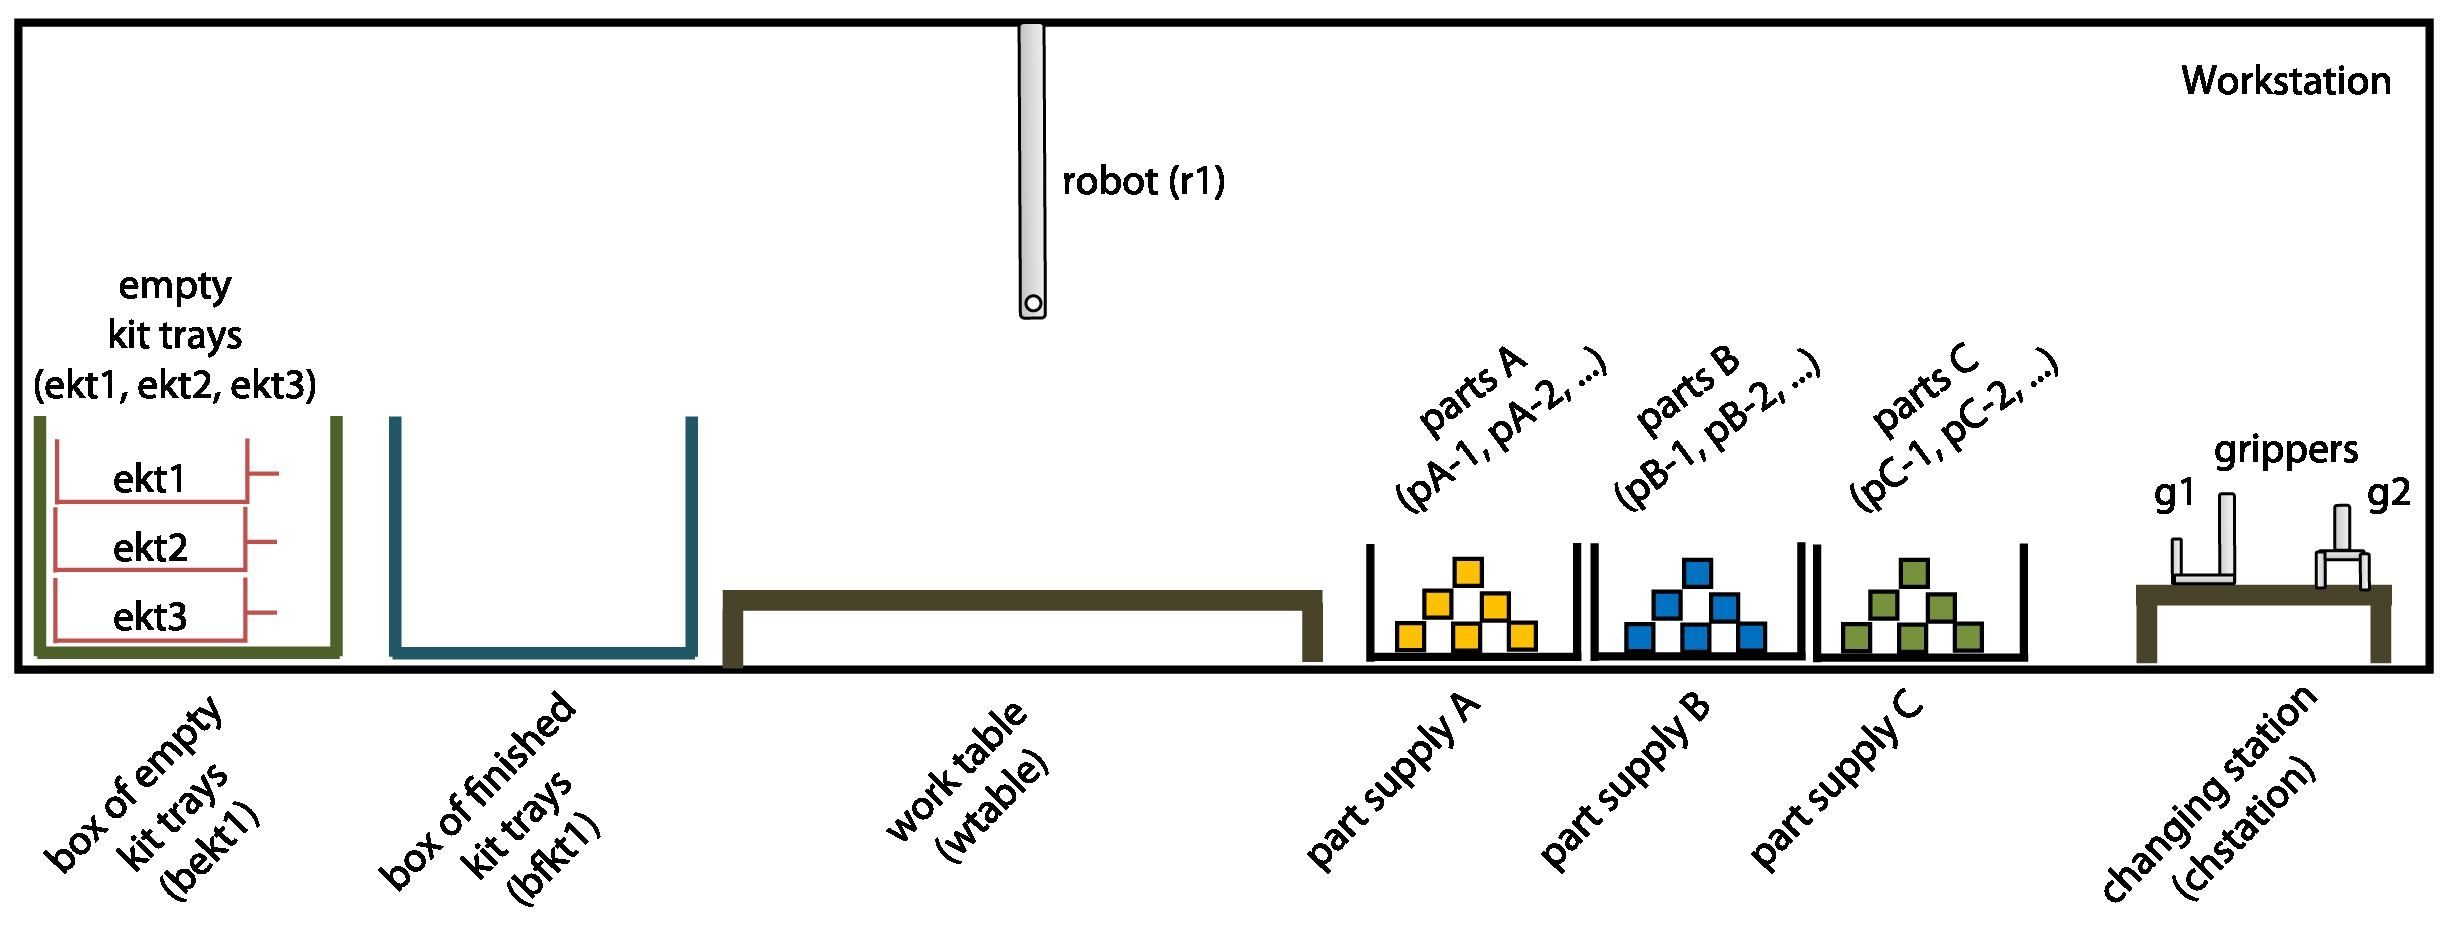
\includegraphics[width=12cm]{Figure/s_initial.jpg}
\caption{Initial state $s_0$.}
\label{fig:initial_state}
\end{figure}

The initial state $s_0$ (see Figure~\ref{fig:initial_state}) is defined as follows:

\begin{itemize}
\item The robot is not holding anything.
\item All the grippers are in the changing station.
\item The box of empty kit trays is not empty.
\item Part supplies are not empty.
\item The box of finished kit trays may contain a number of finished kit tray $n$ with $0\leq n < maxfkt$, where $maxfkt$ is the maximum finished kit trays that can fit in the box of finished kit trays. If the box of finished kit tray is already full, the robot will not be able to place the current finished kit tray in the box of finished kit trays.
\item There is no kit tray on the work table.
\end{itemize}

%The kitting process will fail if there is not at least one empty kit tray in the box of empty kit trays.

$s_0$ can be defined as the following set of ground state variables:
\begin{itemize}
 \item[{\color{RubineRed}$\blacksquare$}] $s_0 = \lbrace$\textit{rhold}(\constant{r1})=$\lbrace nil\rbrace$, \textit{gloc}(\constant{g1})=\chstation, \textit{gloc}(\constant{g2})=\chstation, \textit{boxempty}(\constant{bekt1})=0,\\ \textit{boxempty}(\constant{psA})=0, \textit{boxempty}(\constant{psB})=0, \textit{boxempty}(\constant{psC})=0, \textit{boxfull}(\constant{bfkt1})=0,\\ \textit{topworktable}(\wtable)=$\lbrace nil\rbrace$, \textit{topbox}(\constant{bekt1})=\constant{ekt1}, \textit{ektloc}(\constant{ekt1})=\constant{bekt1}, \textit{ektloc}(\constant{ekt2})=\constant{bekt1}, \textit{ektloc}(\constant{ekt3})=\constant{bekt1}$\rbrace$
\end{itemize}


\subsection{Goal State}

\begin{figure}[h!]
\centering
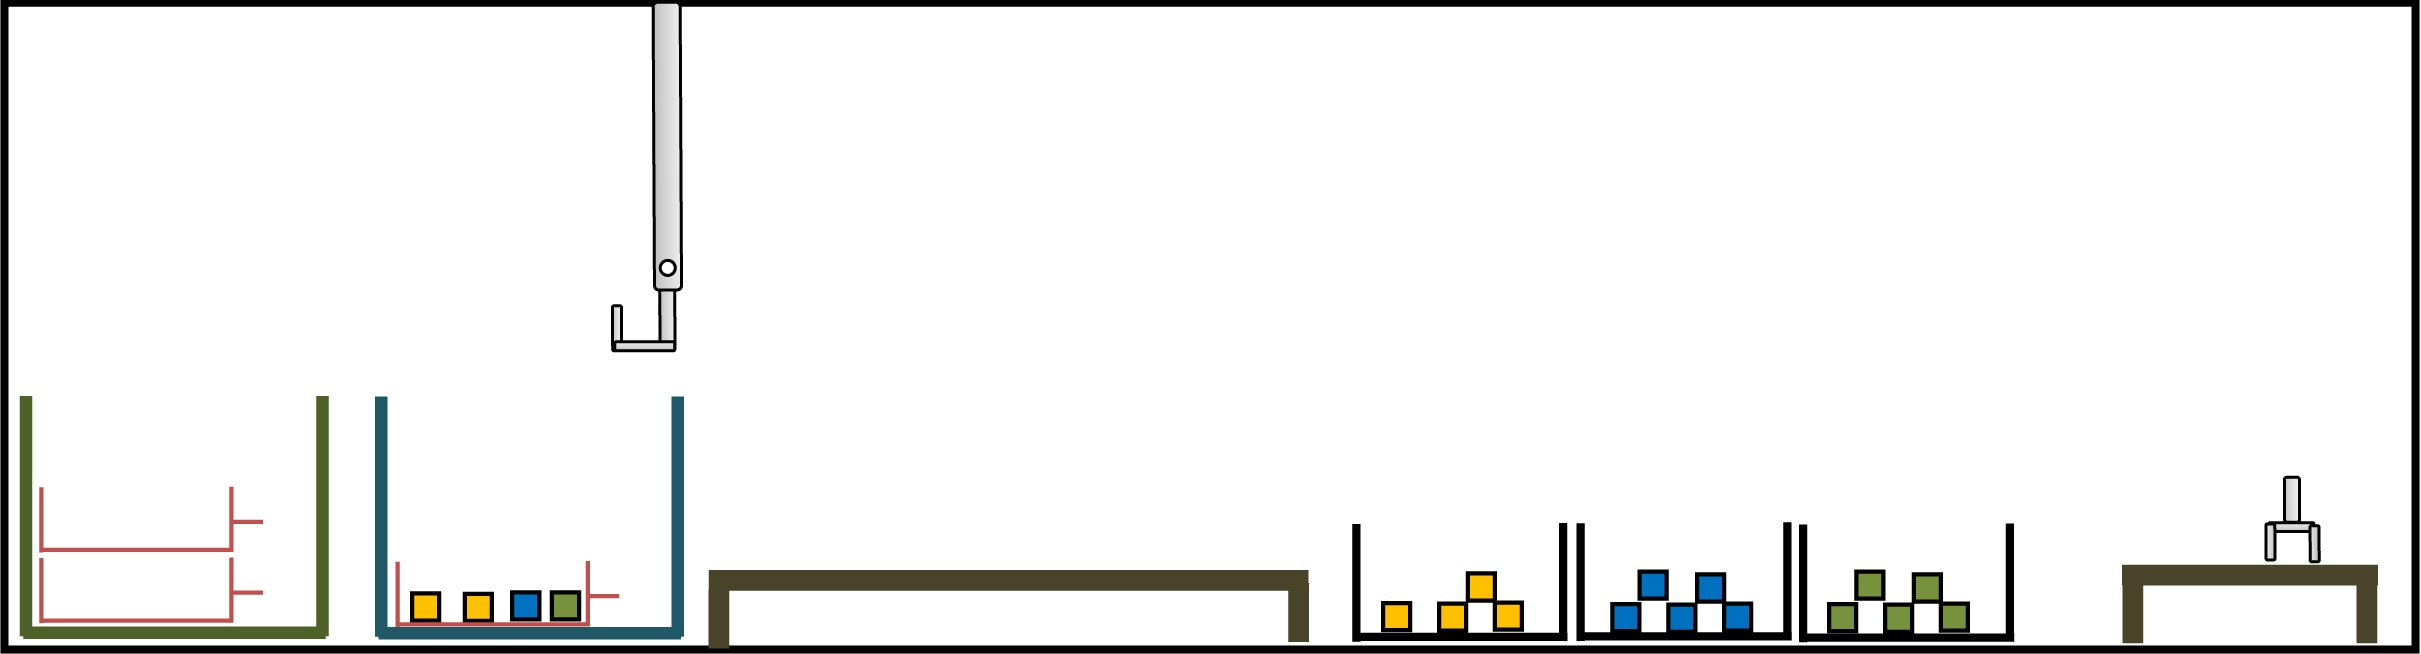
\includegraphics[width=12cm]{Figure/s_goal.jpg}
\caption{Goal state $s_g$.}
\label{fig:goal_state}
\end{figure}

The goal state $s_g$ (see Figure~\ref{fig:goal_state}) is reached when both of the following statements are achieved:

\begin{itemize}
\item The finished kit tray has two parts A, one part B and one part C.
\item The finished kit tray is in the box of finished kit trays.
\end{itemize}

$s_g$ can be defined as the following set of ground state variables:
\begin{itemize}
 \item[{\color{RubineRed}$\blacksquare$}] $s_g$ = $\lbrace$\textit{rhold}(\constant{r1})=$\lbrace nil\rbrace$, \textit{topworktable}(\wtable)=$\lbrace nil\rbrace$, \textit{ploc}(\constant{pA-1})=\constant{fkt1}, \textit{ploc}(\constant{pA-2})=\constant{fkt1}, \textit{ploc}(\constant{pB-1})=\constant{fkt1}, \textit{ploc}(\constant{pC-1})=\constant{fkt1}, \textit{fktloc}(\constant{fkt1})=\constant{bfkt1}$\rbrace$
\end{itemize}





\begin{comment}
\begin{figure}[ht]
\begin{minipage}[b]{0.5\linewidth}
\centering
\includegraphics[scale=0.4]{state/s0.jpg}
\caption{Goal state $s_g$.}
\label{fig:initial_state}
\end{minipage}
\hspace{0.5cm}
\begin{minipage}[b]{0.5\linewidth}
\centering
\includegraphics[scale=0.4]{state/s34.jpg}
\caption{Goal state $s_g$.}
\label{fig:goal_state}
\end{minipage}
\end{figure}


\begin{figure}[ht]
\begin{minipage}[b]{0.5\linewidth}
\centering
\includegraphics[scale=0.4]{Figure/s0.jpg}
\caption{default}
\label{fig:figure1}
\end{minipage}
\hspace{0.5cm}
\begin{minipage}[b]{0.5\linewidth}
\centering
\includegraphics[scale=0.4]{Figure/s1.jpg}
\caption{default}
\label{fig:figure2}
\end{minipage}
\hspace{0.5cm}
\begin{minipage}[b]{0.5\linewidth}
\centering
\includegraphics[scale=0.4]{Figure/s2.jpg}
\caption{default}
\label{fig:figure2}
\end{minipage}
\hspace{0.5cm}
\begin{minipage}[b]{0.5\linewidth}
\centering
\includegraphics[scale=0.4]{Figure/s3.jpg}
\caption{default}
\label{fig:figure2}
\end{minipage}
\hspace{0.5cm}
\begin{minipage}[b]{0.5\linewidth}
\centering
\includegraphics[scale=0.4]{Figure/s4.jpg}
\caption{default}
\label{fig:figure2}
\end{minipage}
\hspace{0.5cm}
\begin{minipage}[b]{0.5\linewidth}
\centering
\includegraphics[scale=0.4]{Figure/s5.jpg}
\caption{default}
\label{fig:figure2}
\end{minipage}
\hspace{0.5cm}
\begin{minipage}[b]{0.5\linewidth}
\centering
\includegraphics[scale=0.4]{Figure/s6.jpg}
\caption{default}
\label{fig:figure2}
\end{minipage}
\hspace{0.5cm}
\begin{minipage}[b]{0.5\linewidth}
\centering
\includegraphics[scale=0.4]{Figure/s7.jpg}
\caption{default}
\label{fig:figure2}
\end{minipage}
\hspace{0.5cm}
\begin{minipage}[b]{0.5\linewidth}
\centering
\includegraphics[scale=0.4]{Figure/s8.jpg}
\caption{default}
\label{fig:figure2}
\end{minipage}
\hspace{0.5cm}
\begin{minipage}[b]{0.5\linewidth}
\centering
\includegraphics[scale=0.4]{Figure/s9.jpg}
\caption{default}
\label{fig:figure2}
\end{minipage}
\hspace{0.5cm}
\begin{minipage}[b]{0.5\linewidth}
\centering
\includegraphics[scale=0.4]{Figure/s10.jpg}
\caption{default}
\label{fig:figure2}
\end{minipage}
\hspace{0.5cm}
\begin{minipage}[b]{0.5\linewidth}
\centering
\includegraphics[scale=0.4]{Figure/s11.jpg}
\caption{default}
\label{fig:figure2}
\end{minipage}
\hspace{0.5cm}
\begin{minipage}[b]{0.5\linewidth}
\centering
\includegraphics[scale=0.4]{Figure/s12.jpg}
\caption{default}
\label{fig:figure2}
\end{minipage}
\hspace{0.5cm}
\begin{minipage}[b]{0.5\linewidth}
\centering
\includegraphics[scale=0.4]{Figure/s13.jpg}
\caption{default}
\label{fig:figure2}
\end{minipage}
\hspace{0.5cm}
\begin{minipage}[b]{0.5\linewidth}
\centering
\includegraphics[scale=0.4]{Figure/s14.jpg}
\caption{default}
\label{fig:figure2}
\end{minipage}
\hspace{0.5cm}
\begin{minipage}[b]{0.5\linewidth}
\centering
\includegraphics[scale=0.4]{Figure/s15.jpg}
\caption{default}
\label{fig:figure2}
\end{minipage}
\end{figure}
\end{comment} 